\documentclass[12pt]{ruthesis}

\usepackage{amsmath}
\usepackage{amssymb}
\usepackage{latexsym}

\usepackage{graphicx}
\usepackage{microtype}

\usepackage{booktabs} % personal preference - can be removed if not using this table style
\usepackage{makecell} % Can be removed if not using this table style

% You can use whatever algorithm environment you want. I used algorthmic here. You can replace this with your own.
\usepackage{algorithm}
\usepackage[noend]{algorithmic}
\usepackage{setspace} % Used to set the line spacing inside the algorithm environment.


\usepackage{epsfig,epsf,rotating}
\usepackage{subfigure}
\usepackage{pictex}
\usepackage{epsf}
\usepackage{cite}
\usepackage{theorem}
\usepackage{amsmath}
\usepackage{amssymb}
\usepackage{amsthm}
\usepackage{bbm} % Not important for template, can be removed if not using bbm inside equations

\newtheorem{theorem}{Theorem}
\newtheorem{lemma}{Lemma}
\newtheorem{definition}{Definition}

\title{Thesis Template in \LaTeX}
\ctitle{Thesis Template}
\author{Benjamin Coleman}
\department{Electrical and Computer Engineering}
\school{Rice University}
\degree{Master of LaTeX}

\committee {
        Professor A, Chair \\
        Assistant Professor of Typography \and
        Professor B  \\
        Assistant Professor of Graphics \and
        Professor C\\
        Professor of Preposterous Formatting Guidelines
}

\address{Houston, Texas}
\donemonth{July} \doneyear{2022} \makeindex
\begin{document}
  \begin{frontmatter}
   \pagenumbering{roman}
   \maketitle
\begin{abstract}
In this work, we develop a thesis template that Rice University Graduate and 

An abstract is to be included with the thesis. Particular care should be taken in preparing the abstract since it will be published in Dissertation Abstracts or Master's Abstracts and the length is limited by the publisher. The abstract may not exceed 350 words for a doctorate or 150 words for a master's. In style, the abstract should be a miniature version of the thesis. It should be a summary of the results, conclusions or main arguments presented in the thesis.

It's pretty unlikely for the abstract to overflow to the following page, if you are following the guidelines. To check that the formatting is correct, we'll simulate this behavior with a \verb_\newpage_ command.
\newpage
If we \textit{do} overflow the abstract onto a new page, then there should not be any page numbers in the top right.

\end{abstract}
   \acknowledge{
   In generating this template, I would like to thank Jan Erik Odegard (who wrote the previous, more complicated version of this template in 1995) and Brent Carey (whose Word 2007 version of the template contained several jokes that we reproduce here).

Use this space to thank the funding and folks that contributed to your success in graduate school. Some view this as an informal section of the thesis, while others still consider this a piece within a formal document. You can thank people like your advisor(s), committee members, peers, friends, family, and even a special pet if you couldn't have done all the late nights without them! Be cautious to not reveal too much sensitive personal information that could be used in identity theft.

Note: Remove the \verb_\newpage_ command when preparing the final document - this is only to check that the page numbering behavior is correct.
\newpage
If we have so many acknowledgements that it overflows onto a new page, then we have to show a page number (using Roman numerals) in the top right.
   }
  \tableofcontents
  \listoffigures
  \listoftables
  \listofalgorithms
  \preface{
  You can optionally include a preface here. This feels a little pretentious, but I say \textit{go for it}. If you don't want to include a preface, then delete this section.
}
  
  \end{frontmatter}
\pagenumbering{arabic}

\linespacing{1.7}

\chapter{Introduction}

There are a couple official Rice University LaTeX templates. The problem is that, as of 2020, these templates no longer compile with modern versions of LaTeX. There are also lots of superfluous style files that are unused and are -- by now -- over 30 years old. In 2022, things are much easier than they were in the 90s.

Specifically, we fixed the graphics and added algorithms. The previous template was unable to include figures and did not list algorithms in the table of contents.

\textbf{Note:} GPS accepted my Master's thesis using this template, so it should be fine for you as well.

\section{Using the Template}
Unlike previous templates, this one only requires \textit{one} .cls file instead of ten .cls and .sty files. That's an order of magnitude fewer files! Just include \verb_ruthesis.cls_ in the same directory as your main LaTeX file and hit compile.

This template has been confirmed to work with Overleaf and TeX Live on MacOS Monterey (as of 2022).

\chapter{Formatting the Text}


\section{Chapter Sections}

\subsection{Subsections}

\subsubsection{Subsubsections}
Note that subsubsections do not appear in the table of contents


\section{Page Numbers}

\subsection{Numbering the Front Matter}

Page numbers should not be shown on the Title Page, the Abstract, or on the first page of the Acknowledgments, Table of Contents, List of Tables or the Preface. However, the following pages (e.g., the second and succeeding pages) of each of these sections should be numbered using Roman numerals. The count for these preliminary pages should start with the title page. For example, if the thesis has a two-page abstract, then the second page of the acknowledgments should be the first page showing a number, and it should be numbered with the Roman numeral v.

\subsection{Numbering the Main Text}

Page numbers should be placed in the upper right corner of the page. Only the number should appear, not ``page 9'' or the abbreviation ``p. 9.'' On the first page of each chapter, the number may be placed at the center bottom, one double space below the last line of type (the conventional placement), or at the top right corner.

Pages of the text itself and of all items following the text (i.e. the notes and bibliography) should be numbered consecutively throughout in Arabic numbers, beginning with number 1 on the first page of the first chapter or introduction (but not preface). Please number every page to be bound, including pages on which only illustrations, drawings, tables, or captions appear. The page numbers do not need to meet the 1'' margin requirements.


\chapter{Formatting Other Stuff}

You will probably have other things in your thesis (tables, figures, etc). Here is how to format those.

\section{Algorithms}

Previous Rice University thesis templates included additional style files to style algorithms. Fortunately, this is no longer necessary. You can use any algorithm environment that you wish. We'll use \verb_algorithmic_ to style Algorithm~\ref{alg:graduation}. Note the use of \verb_setstretch_ to reset the line spacing - if you don't do this, then the algorithm environment will just inherit the double spacing used for the main text (this looks atrocious).

\begin{algorithm}[H]
   \caption{Finish PhD Program}
   \label{alg:graduation}
\setstretch{1.0} % This is necessary so that we don't have double spaced algorithm lines.
\begin{algorithmic}
   \STATE {\bfseries Input:} A student.
   \STATE {\bfseries Output:} A PhD.
   \STATE $N = 0$ number of papers published.
   \WHILE{not graduated}
      \STATE $N = N + 1$
   \ENDWHILE
\end{algorithmic}
\end{algorithm}

Anything within an \verb_algorithm_ environment will appear in the ``Algorithms'' section of the table of contents. If you don't want this for some reason, then you can comment out the \verb_\listofalgorithms_ command in the front matter. 


\section{Tables}

In similar fashion, we do not have to use any particular tabular package or environment, as long as everything lives within \verb_table_ floating environment. You can use whatever you please. I use the \verb_\toprule_, \verb_\midrule_ and \verb_\bottomrule_ commands from the booktabs package because they look nice (Table~\ref{tab:day}).

\begin{table}
\caption{Average day of a Rice graduate student.}
\vspace{2mm}
  \centering
  \begin{tabular}{ c c c c c c}
\toprule
\makecell{Cups of \\Coffee} & Hours in Lab & \makecell{Productive\\ Hours in Lab} & \makecell{Emails \\Received} & \makecell{Internet Videos\\ Watched} & \makecell{Hours at\\ Valhalla} \\
\midrule
3 & 10 & 3 & 56 & 12 & 2+\\
\bottomrule
\end{tabular}
\vspace{-0.2cm}
\label{tab:day}
\vspace{-0.2cm}
\end{table}

\section{Figures}

Any figure that is included in the \verb_figure_ floating environment will be listed in the table of contents.

The template supports rasterized formats (PNG and JPG) as well as vector graphics (PDFs). Note that you'll need to convert SVGs to PDF as \verb_includegraphics_ does not natively support SVG.

As a test, Figure~\ref{fig:valhalla} is a JPG and Figure~\ref{fig:westU} is a PDF.

\begin{figure}[b]
\centering
\vspace{-0.4cm}
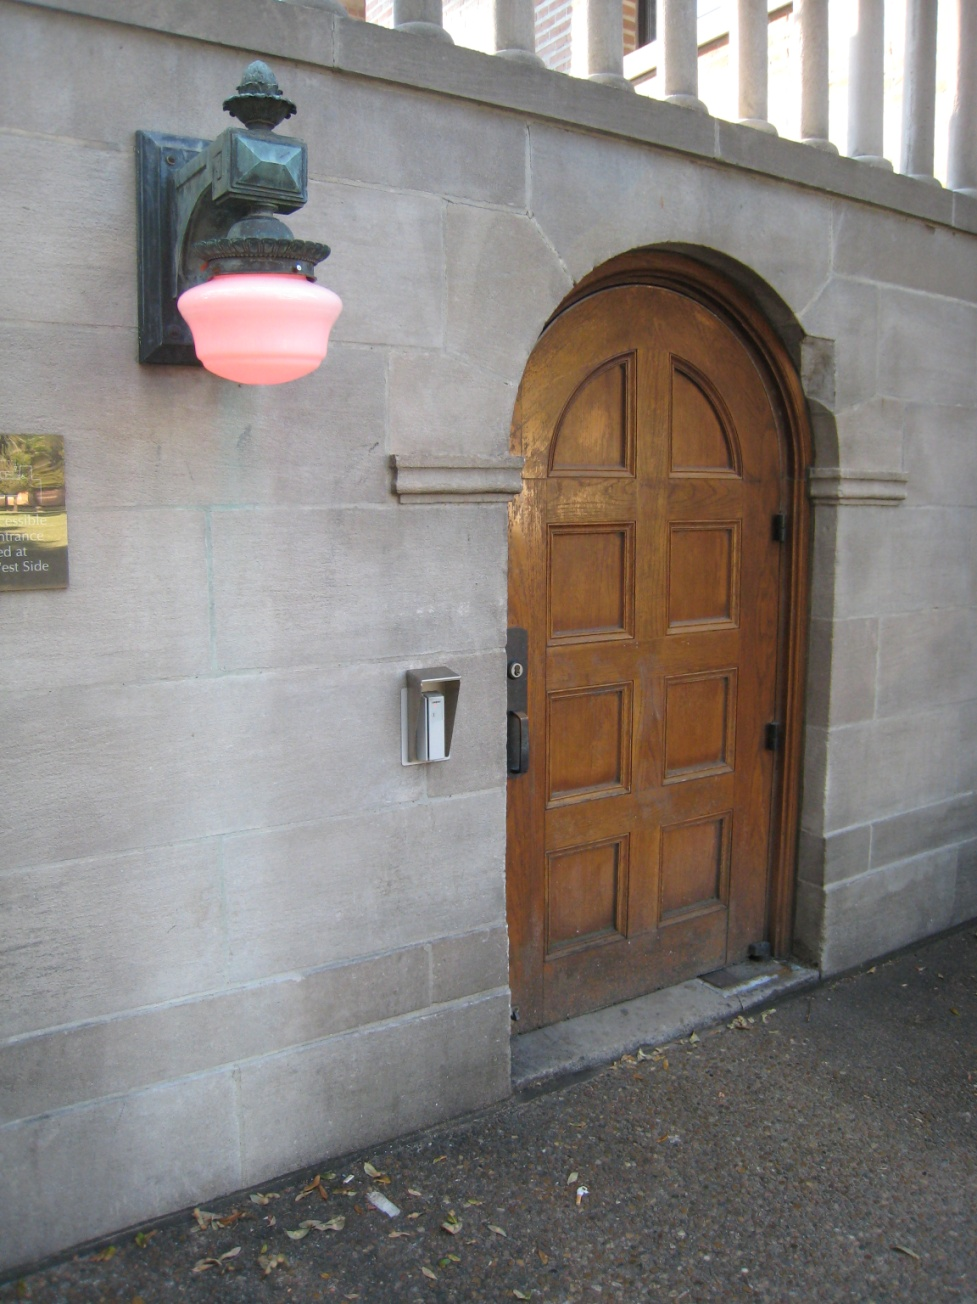
\includegraphics[width=2.5in]{valhalla.jpg}
\caption{My office.}
\label{fig:valhalla}
\end{figure}


\begin{figure}[b]
\centering
\vspace{-0.4cm}
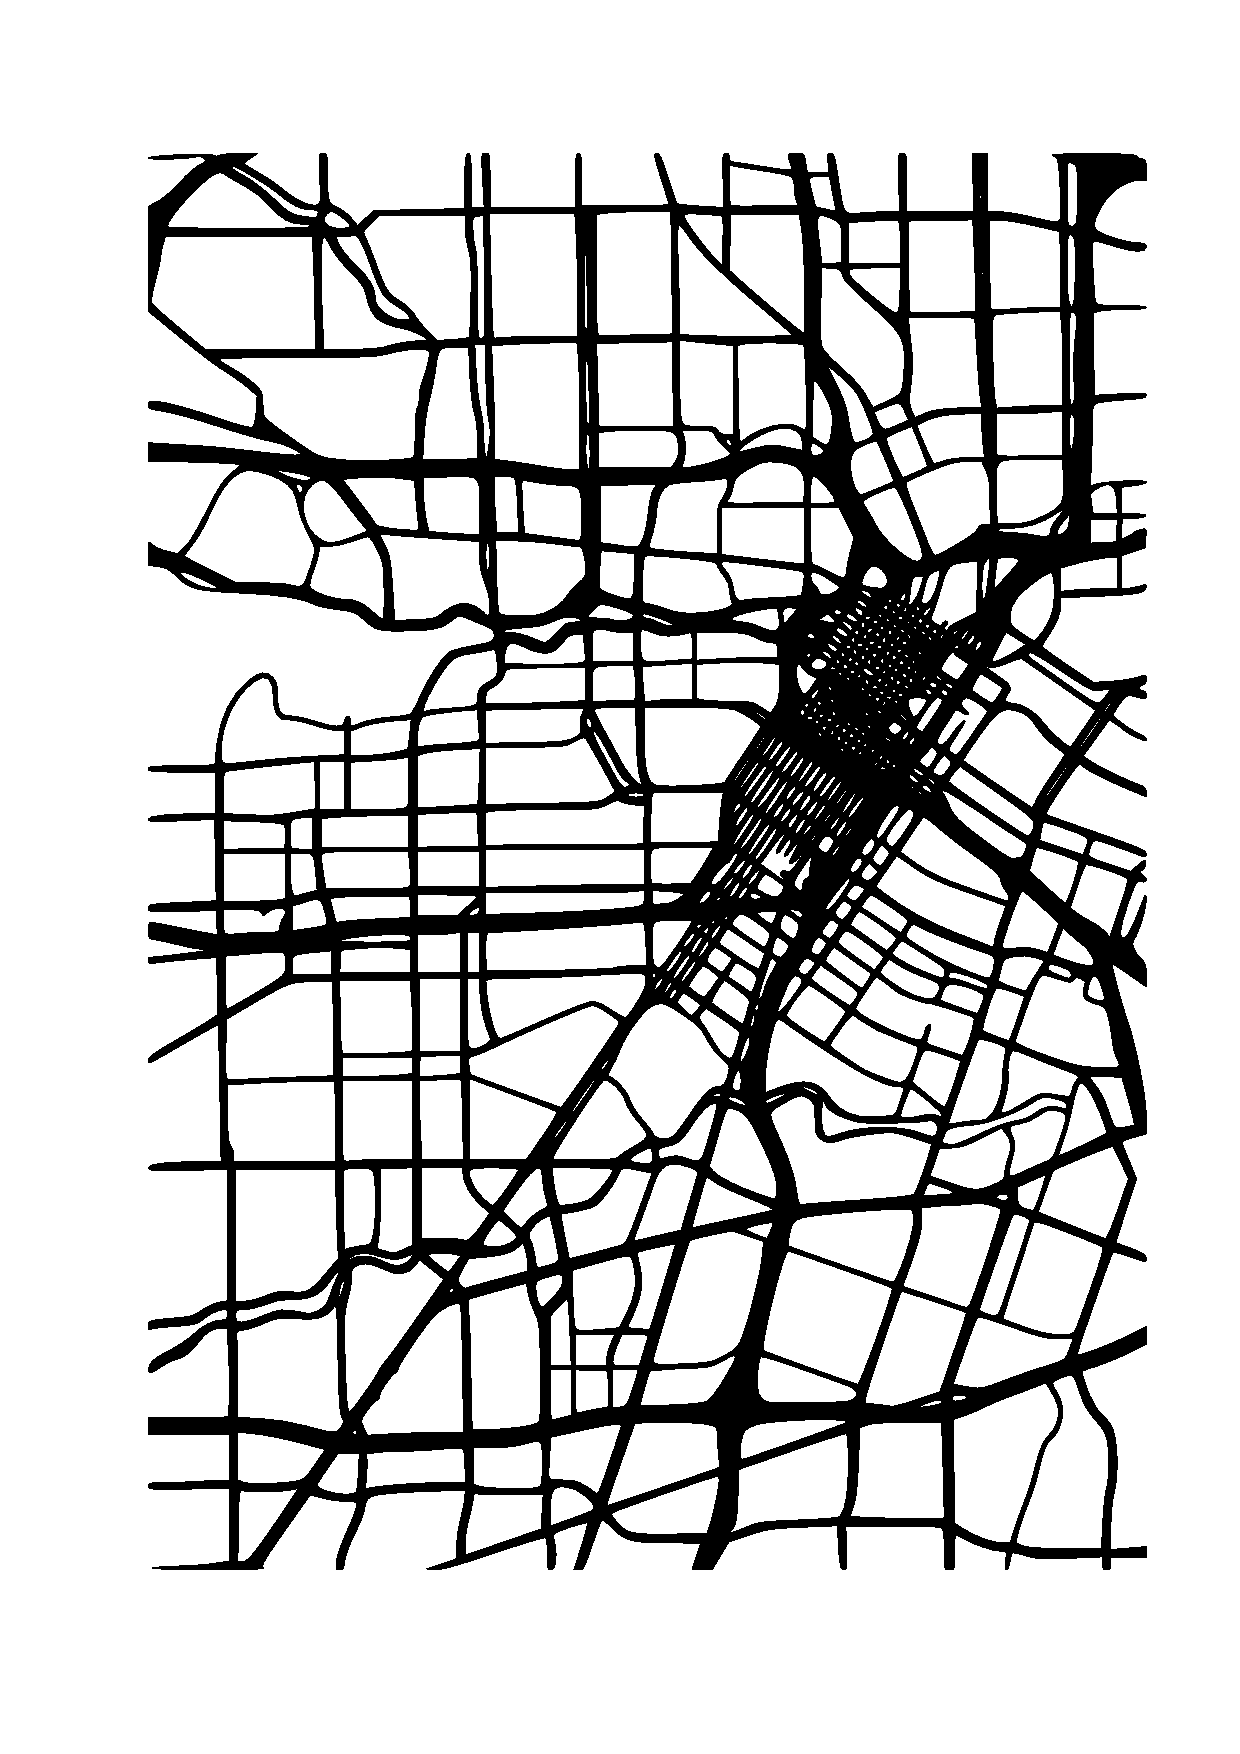
\includegraphics[width=2.5in]{westU.pdf}
\caption{Neighborhood surrounding Rice University (stylized).}
\label{fig:westU}
\end{figure}



\section{Equations}

Numbered equations (Equation~\ref{eq:addition}) are numbered according to the section and subsection.
\begin{equation}
\label{eq:addition}
    1 + 1 = 2
\end{equation}

Non-numbered equations: 
\begin{equation*}
    2 + 2 = 4
\end{equation*}


\subsection{Named Equations}
Would you like to caption equations and then list them in the table of contents? Well too bad! Adding things to the table of contents is easy if the thing is a LaTeX floating environment, but it's not so easy for other things. While we could define a custom custom floating environment that wraps \verb_equation_ for named equations, I'm going to let \textit{you} do that if you want this behavior that badly.

\section{Theorems}

You can use whatever theorem style and environment you want. The default style numbers theorems independently of the section number. This can be changed without modifying the template by specifying \verb_\numberwithin{theorem}{section}_ at the top.

Unfortunately, due to the extremely large margins required by GPS, it is increasingly difficult to ``pull a Fermat.'' Nonetheless, we make our best attempt (Theorem~\ref{thm:fermat}).

\begin{theorem}
\label{thm:fermat}
For any integer $n > 2$, the equation $a^n + b^n = c^n$ has no positive integer solutions.
\end{theorem}
\begin{proof}
The proof is too large to fit into the Texas-sized margins required by GPS and is hence left as an exercise to the reader.
\end{proof}

\section{Citations}
I used the standard IEEE Transactions citation style in my Masters thesis, and it was fine. For example, the proof of Theorem~\ref{thm:fermat} is given by Andrew Wiles~\cite{wiles1995modular}.

\chapter{Conclusion and Future Work}

Go forth and graduate, my friends!

\bibliographystyle{ieeetr}
\bibliography{references}
\end{document}
